\chapter{Samples, setup and experiments}
\label{ch:experiments}

All the experiments have been made on samples manufactured for the IRIS project.
This is due to the fact that in the time frame of this work there would have not been enough time to design and produce an ad hoc device.
Moreover, as already stated, the aim of this thesis is to produce a proof of concept for an all-optical implementation of an activation function, rather than to construct a complete prototype.

\section{The samples}
%The samples used in this work have been provided by the IRIS project.
The IRIS project studied the design and the implementation of an integrated reconfigurable silicon photonics switch matrix, a routing device, as a replacement for electronic devices used in the telecommunication industry.
The completed integrated photonic circuit consists of a matrix of waveguides crossing each other and linked by couples of racetrack resonators, thermally-controlled.
At the ends of the waveguides other structures, interleavers and AWGs, allowed many signals at different wavelengths to be multiplexed/demultiplexed on/from the same waveguide.

The complexity of such photonic circuit required the fabrication, for testing purposes, of each and every structure of which it is composed, with various production parameters.
The collection of all these devices on a chip was produced in many samples.
Isolated from the others, but also grouped together with few other elements.
Specifically these test structures were disposed on a single chip and were accessible via grating couplers.


Since this work is at the beginning of the project, my choice was a system of intermediate complexity, so that it could be used both to test the activation function and the weighted sum.

The structure selected is the following: a simple waveguide, coupled to eight drop channels by a single or a couple of ring resonators each, nicknamed \textit{mini-matrix}.
In this family of devices, there were those built with single microrings, double microrings, single racetracks, or double racetracks.
The final choice was to study the \textit{mini-matrix} in which the coupling mechanism was provided by single ring resonators, because of its simpler transfer function in respect to double microrings or double racetracks.

Moreover, these samples were manufactured with thermo-electric \large\textbf{this is not the correct term} \normalsize pads to heat the rings and effectively tune their resonance.

\begin{figure}[ht]
	\centering
	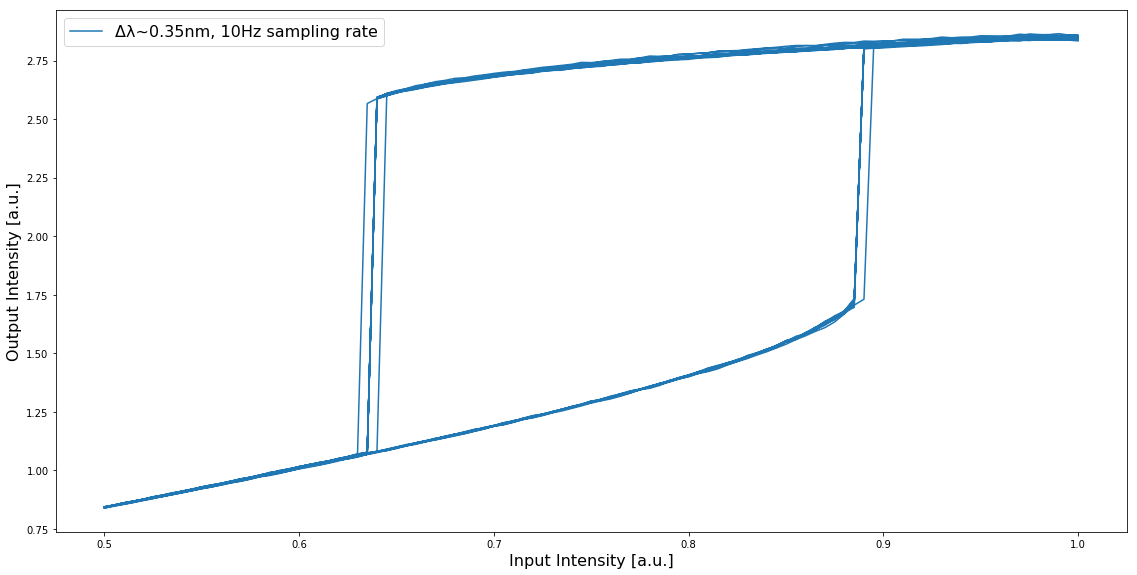
\includegraphics[draft,width=9cm,height=6cm]{figures/foo.png}
	\caption{image/scheme of the minimatrix}
	\label{fig:minimatrix_full}
\end{figure}

\section{Setup}

\section{Characterization of the Activation Function}
\label{sec:Characterization_of_the_Activation_Function}
Characterization of the activation function

\section{Test of a Trained ANN}
\label{sec:Test_of_a_Trained ANN}
Test of the activation function